
\section{Preliminary Concepts}

\subsection{Formulation of the Problem}

\label{sec:statement_of_the_problem}\index{DSE}

Let $S$ be a parameterized system with $n$ parameters. The generic
parameter $p_i, \ i \in \{1,2,\ldots,n\}$ can take any value in
the set $V_i$. A {\em configuration} $\mathbf{c}$ of the system
$S$ is a $n$-tuple $\langle v_1,v_2,\ldots,v_n \rangle$ in which
$v_i \in V_i$ is the value fixed for the parameter $p_i$. The {\em
configuration space} (or {\em design space}) of $S$ [which we will
indicate as $\mathcal{C}(S)$] is the complete range of possible
configurations [$\mathcal{C}(S) = V_1 \times V_2 \times \ldots
\times V_n$]. Naturally not all the configurations of
$\mathcal{C}(S)$ can really be mapped on $S$. We will call the set
of configurations that can be physically mapped on $S$ the {\em
feasible configuration space} of $S$ [and indicate it as
$\mathcal{C}^*(S)$].

Let $m$ be the number of objectives to be optimized (e.g. power,
cost, performance, etc.). An {\em evaluation function}
$E:\mathcal{C}^*(S)\times \mathcal{B} \longrightarrow \Re^m$ is a
function that associates each feasible configuration of $S$ with
an $m$-tuple of values corresponding to the objectives to be
optimized when any application belonging to the set of benchmarks
$\mathcal{B}$ is executed.

Given a system $S$, an application $b \in \mathcal{B}$ and two
configurations $\mathbf{c}', \mathbf{c}'' \in \mathcal{C}^*(S)$,
$\mathbf{c}'$ is said to {\em dominate} (or {\em eclipse})
$\mathbf{c}''$, and is indicated as $\mathbf{c}' \succ
\mathbf{c}''$, if given $\mathbf{o}'=E(\mathbf{c}', b)$ and
$\mathbf{o}''=E(\mathbf{c}'', b)$ it results that $\mathbf{o}'
\leq \mathbf{o}''$ and $\mathbf{o}' \neq \mathbf{o}''$. Where
vector comparisons are interpreted component-wise and are true
only if all of the individual comparisons are true ($o'_i \leq
o''_i \ \forall \ i = 1,2,\ldots,m$).

The {\em Pareto-optimal set} of $S$ for the application $b$ is the
set:
\[ \mathcal{P}(S,b) = \{ \mathbf{c} \in \mathcal{C}^*(S) \ : \nexists \ \mathbf{c}' \in \mathcal{C}^*(S), \mathbf{c}' \succ \mathbf{c} \} \]
that is, the set of configurations $\mathbf{c} \in
\mathcal{C}^*(S)$ not dominated by any other configuration.
Pareto-optimal configurations are configurations belonging to the
Pareto-optimal set and the {\em Pareto-optimal front} is the image
of the Pareto-optimal configurations, i.e. the set:
\[ \mathcal{P}_{F}(S,b) = \{ \mathbf{o} : \mathbf{o} = E(\mathbf{c},b), \mathbf{c} \in \mathcal{P}(S,b) \} \]

The aim of a Design Space Exploration (DSE) strategy is to give a
good approximation of the Pareto-optimal front for a system $S$ and an
application $b$, simulating as few configurations as possible.

%----------------------------------------------------------------



On the contrary, we call ``parameter space representation'' of the
Pareto set the representation in which each configuration $\mathbf{p}$
is simply represented as a point of $P_{1}\times\dots\times P_{n}$
space. We will investigate the relation between the ``objective space
representation'' and the ``parameter space representation''. We
are particularly interested in the relation between the evolution
of the objective space representation of the Pareto set and the evolution
of its parameter space representation.

\begin{figure}[h]
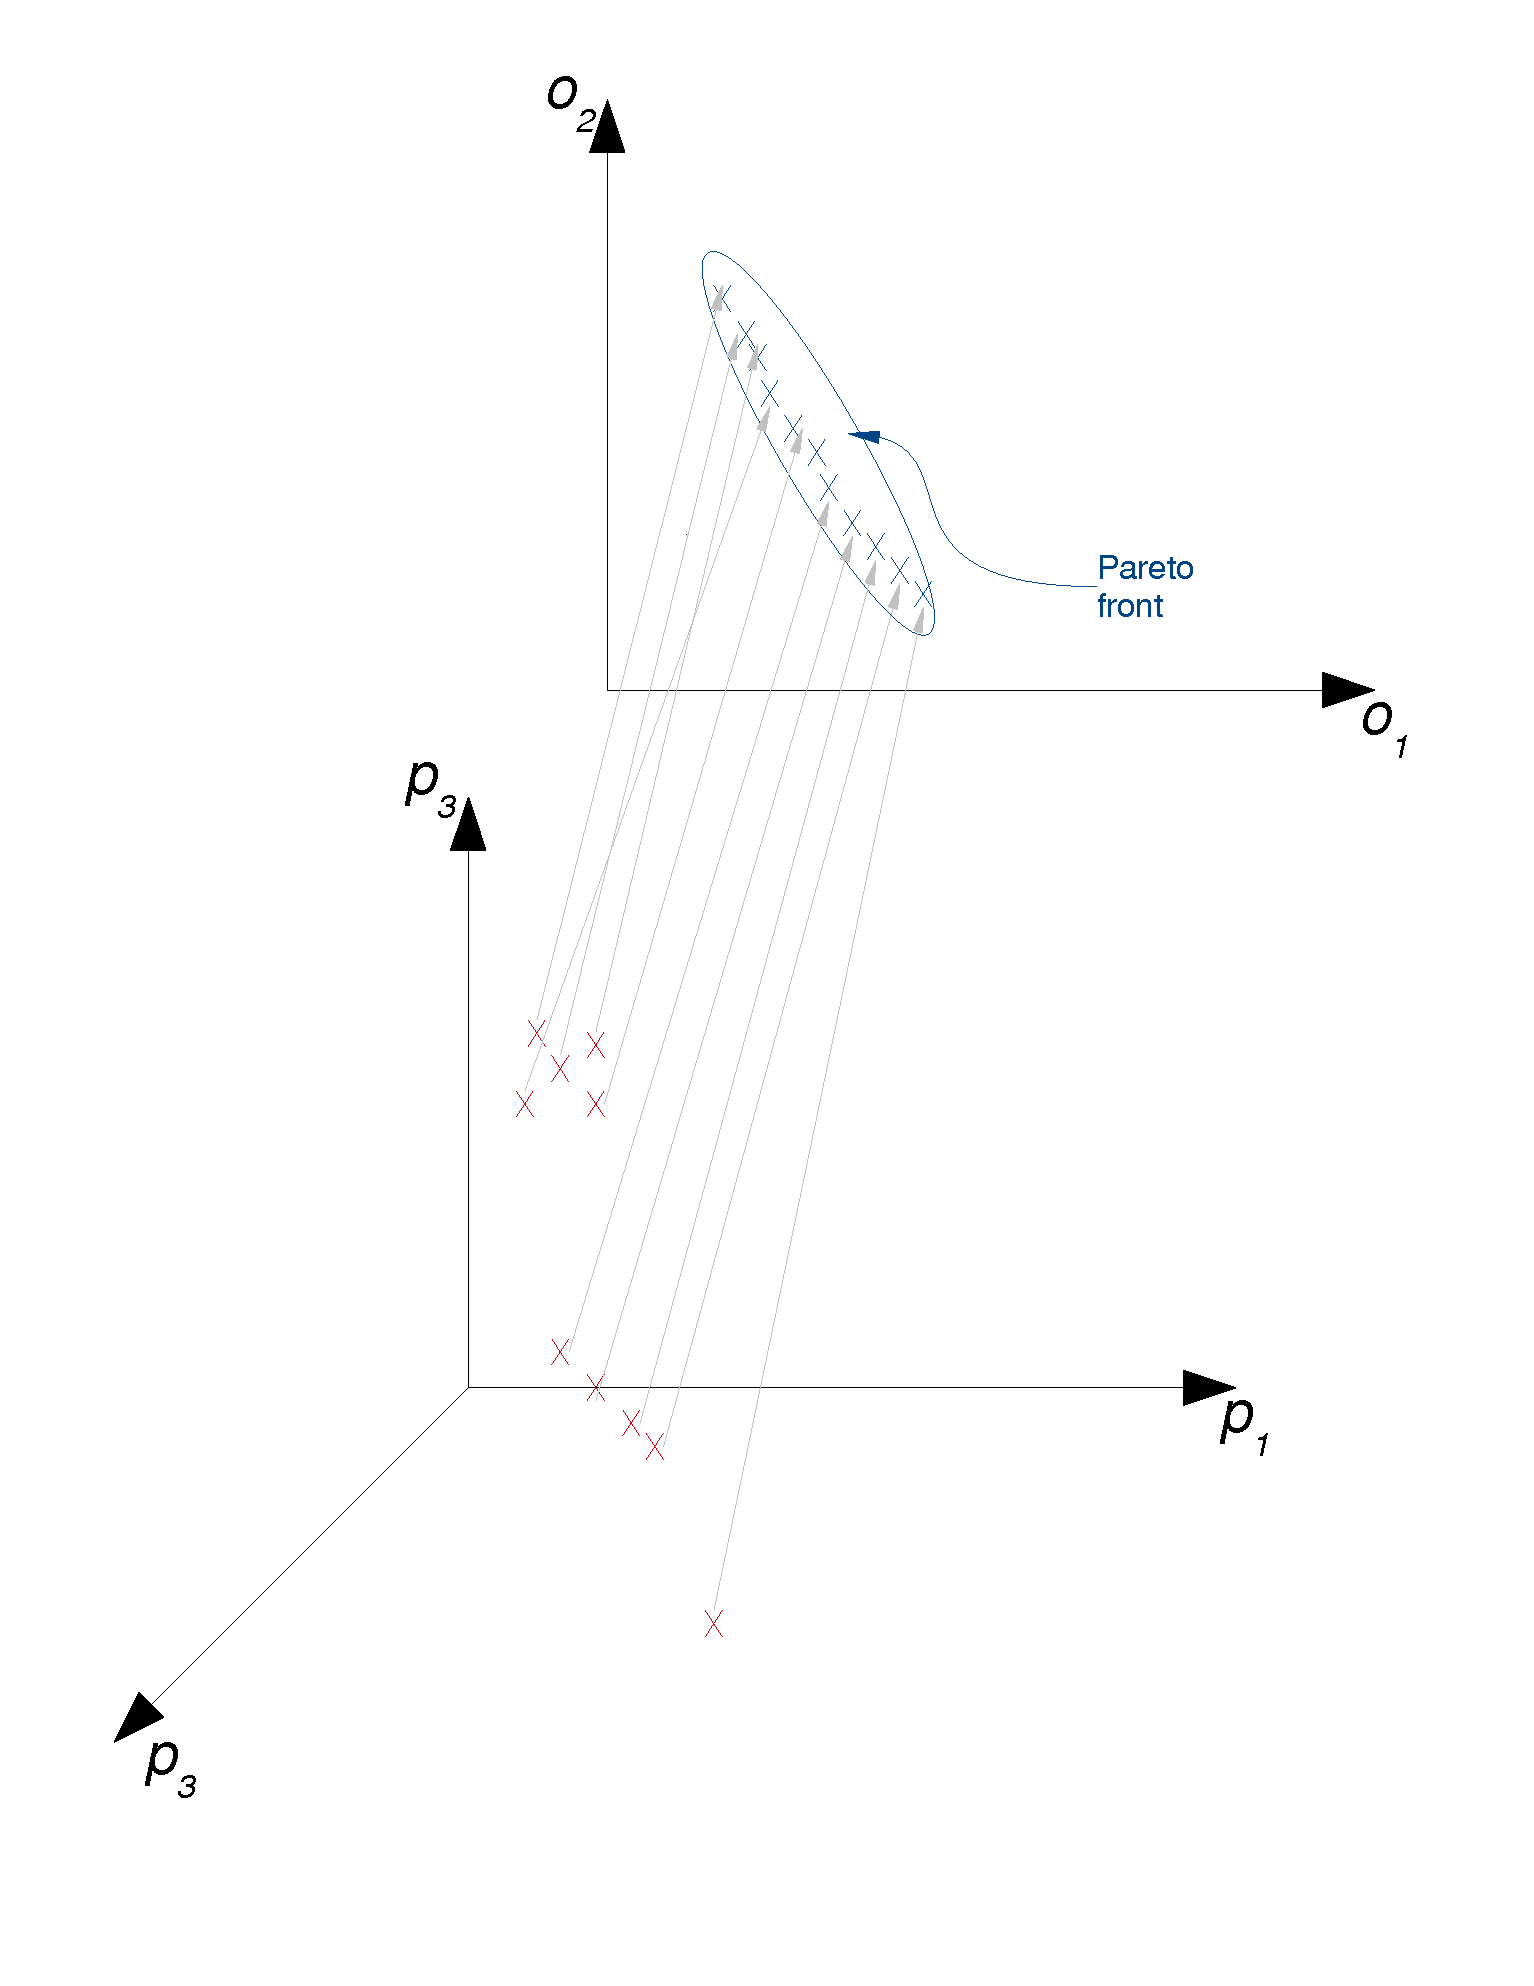
\includegraphics[width=0.9\columnwidth]{img/Pareto_set_and_front}

\caption{Relation between Pareto set (its ``parameter space representation'')
and Pareto front (``objective space representation'')}


\end{figure}

\subsection{Required Definitions and Concepts}

In the design process, there are often a lot of ``local decisions''
in which the designer can take advantage of well-known results or
heuristics. For example, in a VLIW architecture consider a configuration
with very few registers. It is well-known that, in such a condition,
increasing the number of ALUs doesn't lead to tangible better performances
but leads to an increase in area occupation. An intelligent exploration
algorithm wouldn't waste time evaluating configurations with many
ALUs and few registers. If $p_{1}$ is the parameter ``number of
registers'' and $p_{2}$ is the parameter ``number of ALUs'', we
can say that the region:
\[
R=\left\{ \left.\left(v_{1},v_{2}\right)\in P_{1}\times P_{2}\right|v_{1}<s_{1},v_{2}>s_{2}\right\} 
\]
 (where $s_{1}$ and $s_{2}$ are some threshold values) is of little
interest. This example shows that some ``dependency relation'' between
parameters may exist and can be exploited to guide the exploration:
the dependencies between parameters can suggest to the designer that,
if a parameter lies in a range, there are ranges of the other there
aren't worth exploring. Intuitively, the Cartesian product of these
ranges is an ``uninteresting region''.

The problem is that, in complex scenarios, not all relations of this
kind are known in advance. Some dependency may exist but may be hidden
to the designer. Or there may be ``local dependencies'', i.e. two
parameters may be related by a dependency but only if their values
lie on some ranges (so we can't treat them as they were related by
a true dependency). Therefore, as stated in section \ref{sec:Related-work},
setting up an exploration trying to take into account as much dependencies
as possible is a very hard task that is destined to be incompletely
accomplished. We need a methodology to ``automatically'' recognize
interesting or uninteresting regions without requiring a priori knowledge
to the designer.

We also consider, in measuring how much iteresting a region is, the
``innovation'' that it adds. If, during a design space exploration,
a Pareto front is temporarily calculated, adding a new Pareto front
point near to the previous ones is not a considerable ``innovation'',
because the way it fulfils the objectives is very similar to other
already evaluated configurations. On the contrary, adding a new Pareto
front point that is very distant from previous ones is remarkable,
because it let the experimenter realize that the objectives can be
fulfilled in a completely different way from what he already found
during exploration. So a region will be evaluated ineresting as much
as how different are its added Pareto front points from the ones already
found.
\begin{rem}
We will consider only parameters $p_{i}$ with ordering, i.e. such
that, if $P_{i}$ is a domain, $\forall a,b\in P_{i}$ it is possible
to say $a<b$ or $a=b$ or $a>b$.
\end{rem}
%TODO: DESCRIVERE COME SI PENSA DI TRATTARE GLI SCENARI IN CUI ESISTONO
%PARAMETRI SENZA ORDINAMENTO{]}
\begin{defn}
\emph{Parameter interval}

Let $p_{i}$ be a parameter and $a_{i},b_{i}\in P_{i},a_{i}<b_{i}$.
A $p_{i}$- interval is
\[
\left[a_{i}..b_{i}\right]=\left[a_{i},b_{i}\right]\cap P_{i}
\]
 (i.e. taking the interval $\left[a_{i},b_{i}\right]$ , $\left[a_{i}..b_{i}\right]$
is the set of values of $P_{i}$ lying in $\left[a_{i},b_{i}\right]$)
\end{defn}

\begin{defn}
\emph{\label{pers02.def:Contiguous-intervals}Contiguous intervals}

Let $\left[a_{i}..b_{i}\right]$ and $\left[x_{i}..y_{i}\right]$
be two $p_{i}$-intervals. They are said to be contiguous iff
\begin{itemize}
\item $\left[a_{i}..b_{i}\right]\cap\left[x_{i}..y_{i}\right]=\emptyset$
and
\item $\left[a_{i}..b_{i}\right]\cup\left[x_{i}..y_{i}\right]$ is a $p_{i}$-
interval or $\left[x_{i}..y_{i}\right]\cup\left[a_{i}..b_{i}\right]$
is a $p_{i}$- interval
\end{itemize}
\end{defn}
\begin{figure}[h]
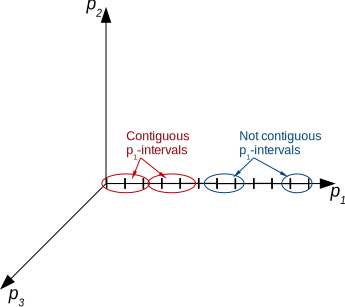
\includegraphics[width=0.9\columnwidth]{img/contiguous_intervals_or_not}

\caption{Examples of contiguous and not contiguous intervals}

\end{figure}

\begin{defn}
\emph{Region}

A region is a set of the following form:
\[
R=\left[a_{1}..b_{1}\right]\times\dots\times\left[a_{n}..b_{n}\right]=\prod\left[a_{i}..b_{i}\right]
\]
 (see figure \ref{pers02.fig:Examples-of-regions})

\begin{figure}[h]
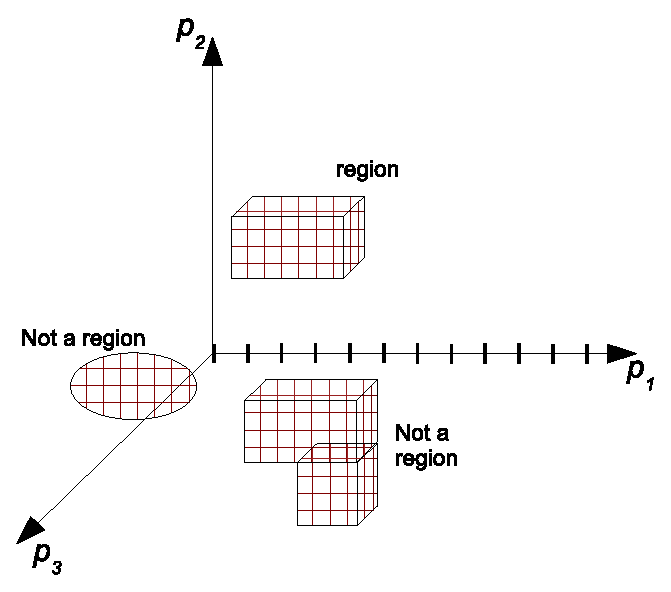
\includegraphics[width=0.9\columnwidth]{img/regions}

\caption{\label{pers02.fig:Examples-of-regions}Examples of regions}


\end{figure}
\end{defn}
\begin{rem}
We will talk later of ``big'' and ``small'' regions. The sense
of these terms is related to the cardinality of regions. A region
$R_{1}$ is said to be \emph{bigger }then $R_{2}$, if
\[
\left|R_{1}\right|>\left|R_{2}\right|
\]
 where $\left|R_{1}\right|$ and $\left|R_{2}\right|$ are the cardinalities
of $R_{1}$ and $R_{2}$. Similarly, a $p_{i}$-interval $\left[a_{i}..b_{i}\right]$
is said to be bigger then another $p_{i}$-interval $\left[c_{i}..d_{i}\right]$
if:
\[
\left|\left[a_{i}..b_{i}\right]\right|>\left|\left[c_{i}..d_{i}\right]\right|
\]


Therefore, the width of a $p_{i}$-interval $\left[a_{i}..b_{i}\right]$
is not given by the numeric value $b_{i}-a_{i}$ but it is its cardinality.
\end{rem}
We now provide some rules to split and merge regions. They will be
useful when explaining our proposed exploration algorithm.
\begin{defn}
\emph{\label{pers02.def:Splitting-a-region}Splitting a region}

If $\left[a_{i}..b_{i}\right]$ has more than one element, i.e. $\left|\left[a_{i}..b_{i}\right]\right|>1$,
it can be split in two contiguous intervals
\[
\left[a_{i}..c_{i}\right],\left[d_{i}..b_{i}\right]
\]
 such that
\[
\begin{cases}
\left[a_{i}..c_{i}\right]\cap\left[d_{i}..b_{i}\right] & =\emptyset\\
\left[a_{i}..c_{i}\right]\cup\left[d_{i}..b_{i}\right] & =\left[a_{i}..b_{i}\right]\\
\left|\left[a_{i}..c_{i}\right]\right| & =\left\lceil \frac{\left|\left[a_{i}..b_{i}\right]\right|}{2}\right\rceil 
\end{cases}
\]


If $\left|\left[a_{i}..b_{i}\right]\right|=1$ instead, the interval
cannot be split. 

If $\left[a_{i}..b_{i}\right]$ can be split, we define
\[
I_{i}=\left\{ \left[a_{i}..c_{i}\right],\left[d_{i},b_{i}\right]\right\} 
\]
 else
\[
I_{i}=\left\{ \left[a_{i}..b_{i}\right]\right\} 
\]


The whole region can be split in the following subregions
\[
\mathcal{R}^{R}=\left\{ \left.\prod\left[x_{i}..y_{i}\right]\right|\left[x_{i}..y_{i}\right]\in I_{i}\right\} 
\]


See figure \ref{pers02.fig:Splitting-a-region}.

\begin{figure}[h]
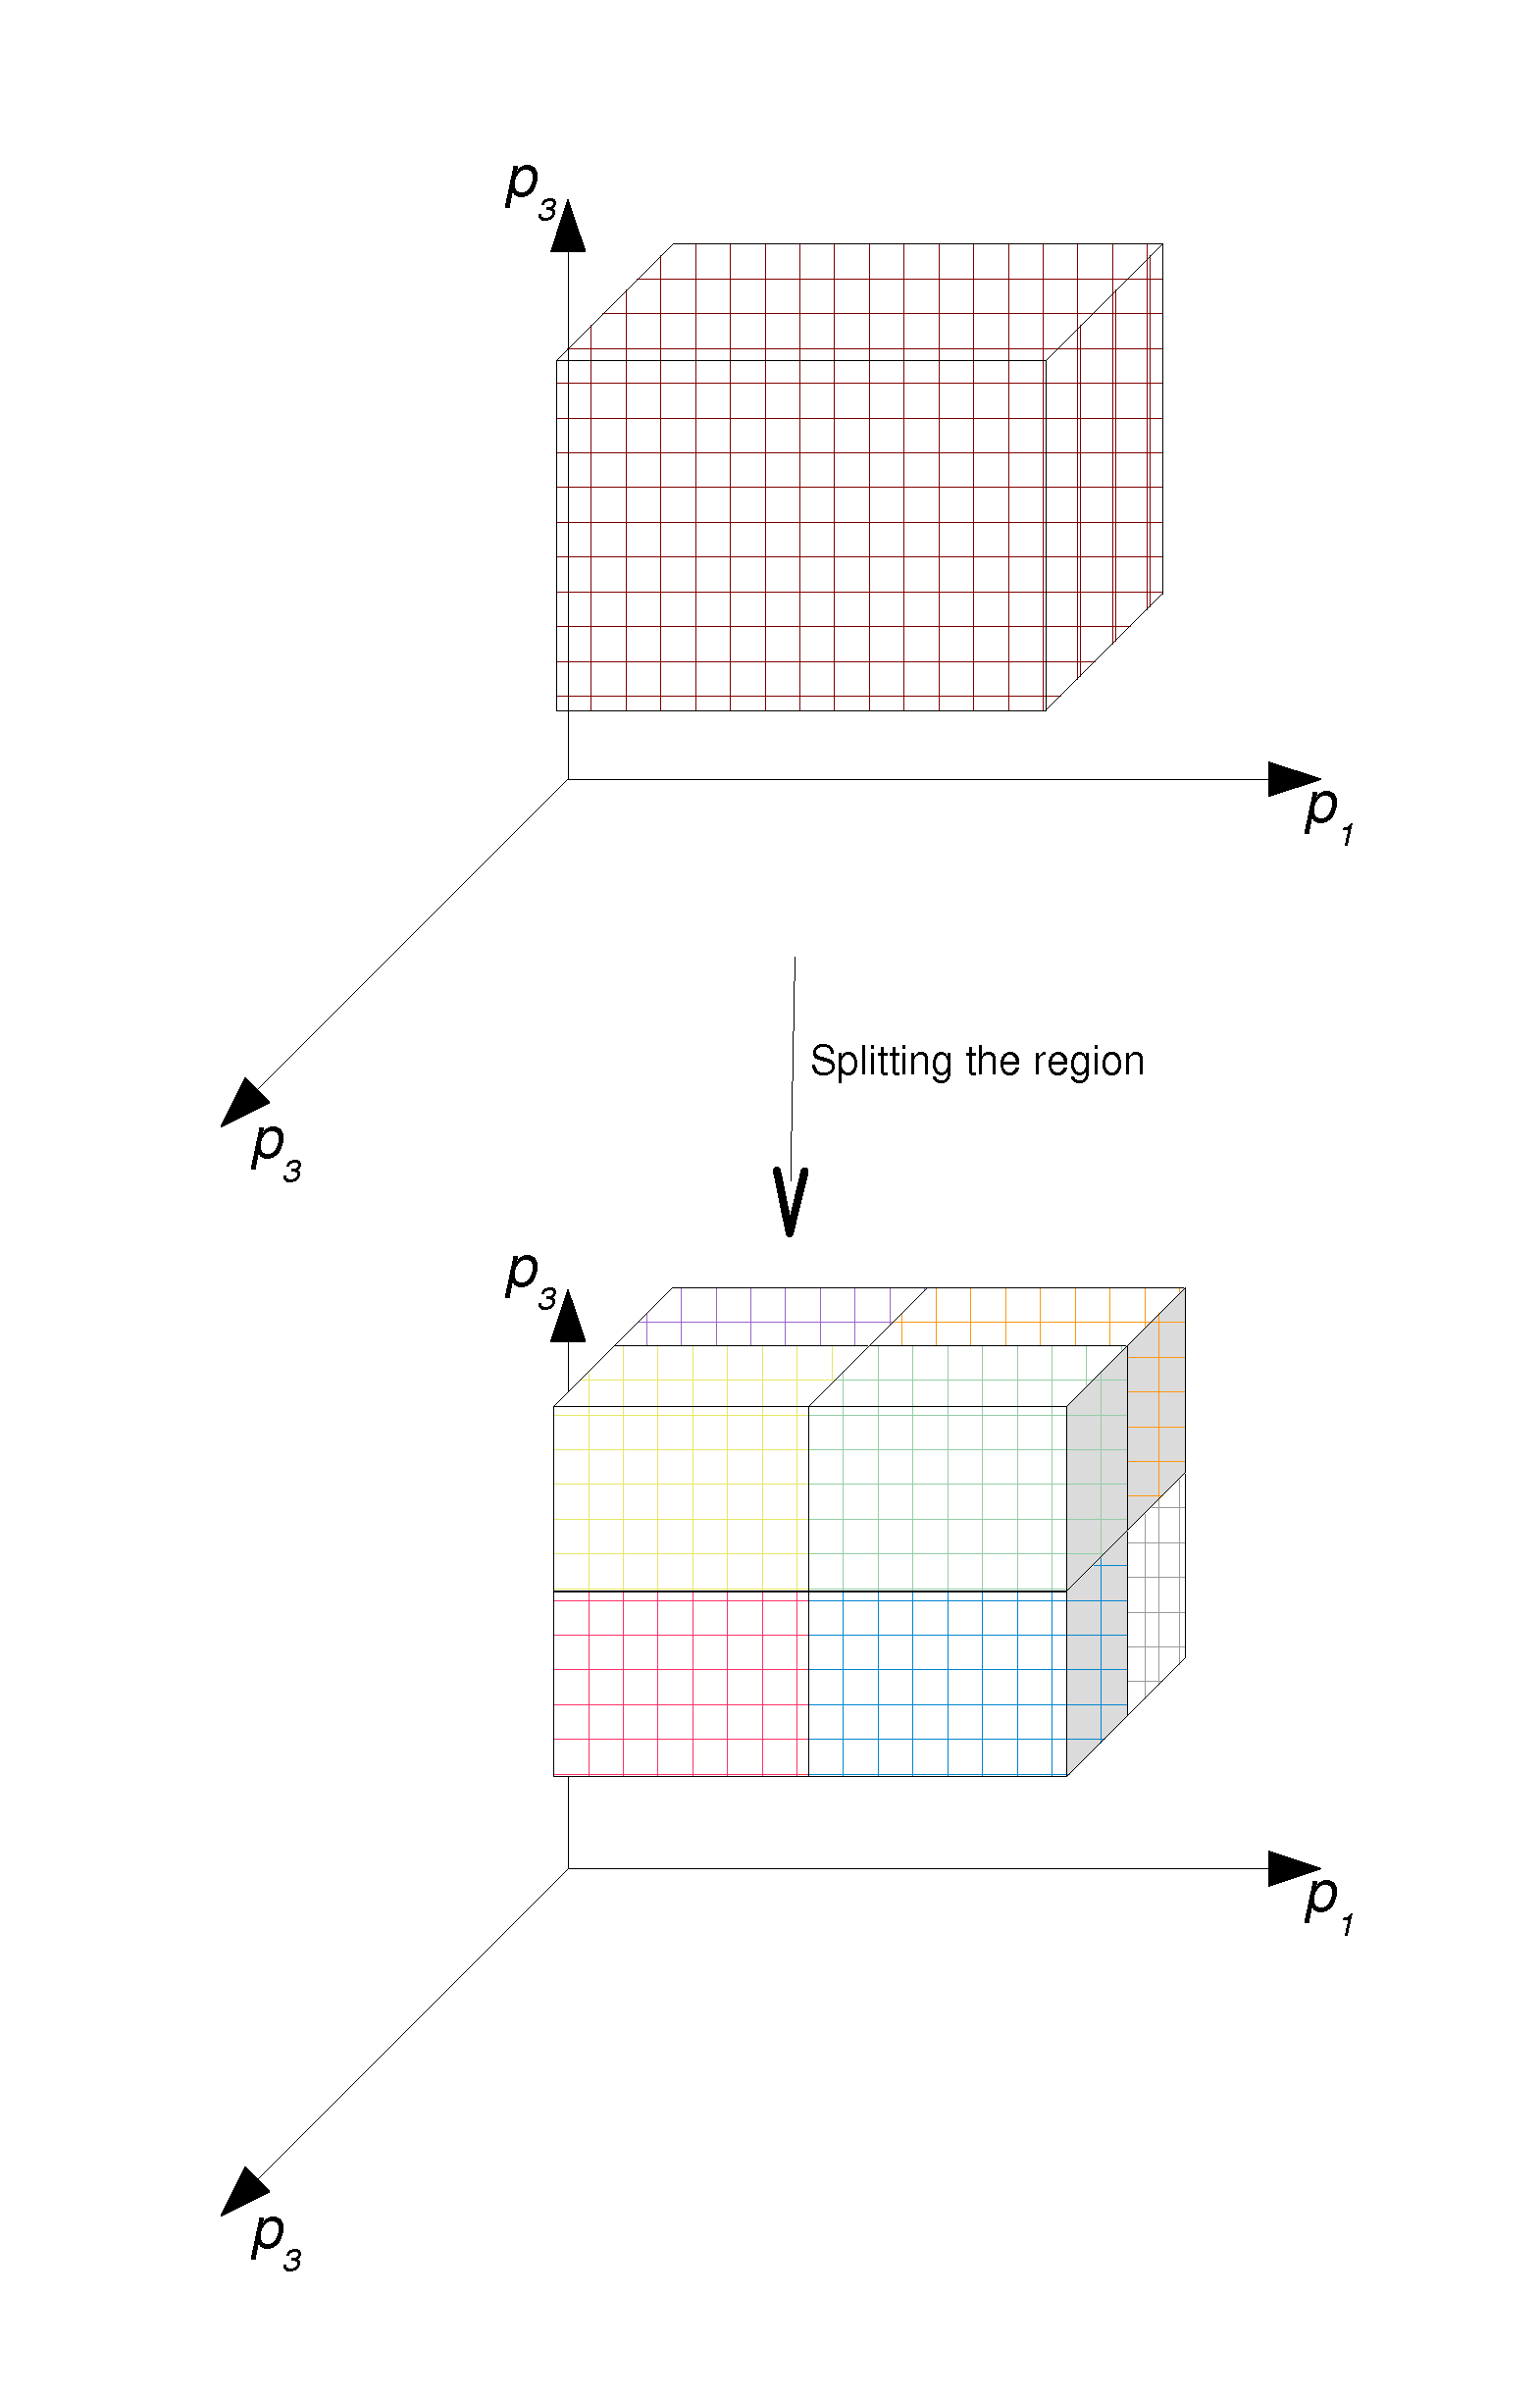
\includegraphics[width=0.9\columnwidth]{img/splitting_the_region}

\caption{\label{pers02.fig:Splitting-a-region}Splitting a region}


\end{figure}

\end{defn}

\begin{defn}
\emph{Contiguous regions}

Let $R_{1}=\prod\left[a_{i}\dots b_{i}\right]$ and $R_{2}=\prod\left[x_{i}..y_{i}\right]$
be two regions. They are said to be contiguous iff
\begin{itemize}
\item a $j$ exists such that $\left[a_{i}..b_{i}\right]=\left[x_{i}..y_{i}\right]$
for all $i\neq j$ 
\item $\left[a_{j}..b_{j}\right]$ and $\left[x_{j}..y_{j}\right]$ are
contiguous intervals (see definition \ref{pers02.def:Contiguous-intervals})
\end{itemize}
\end{defn}
See figure \ref{pers02.fig:Contiguous-regions}.

\begin{figure}[h]
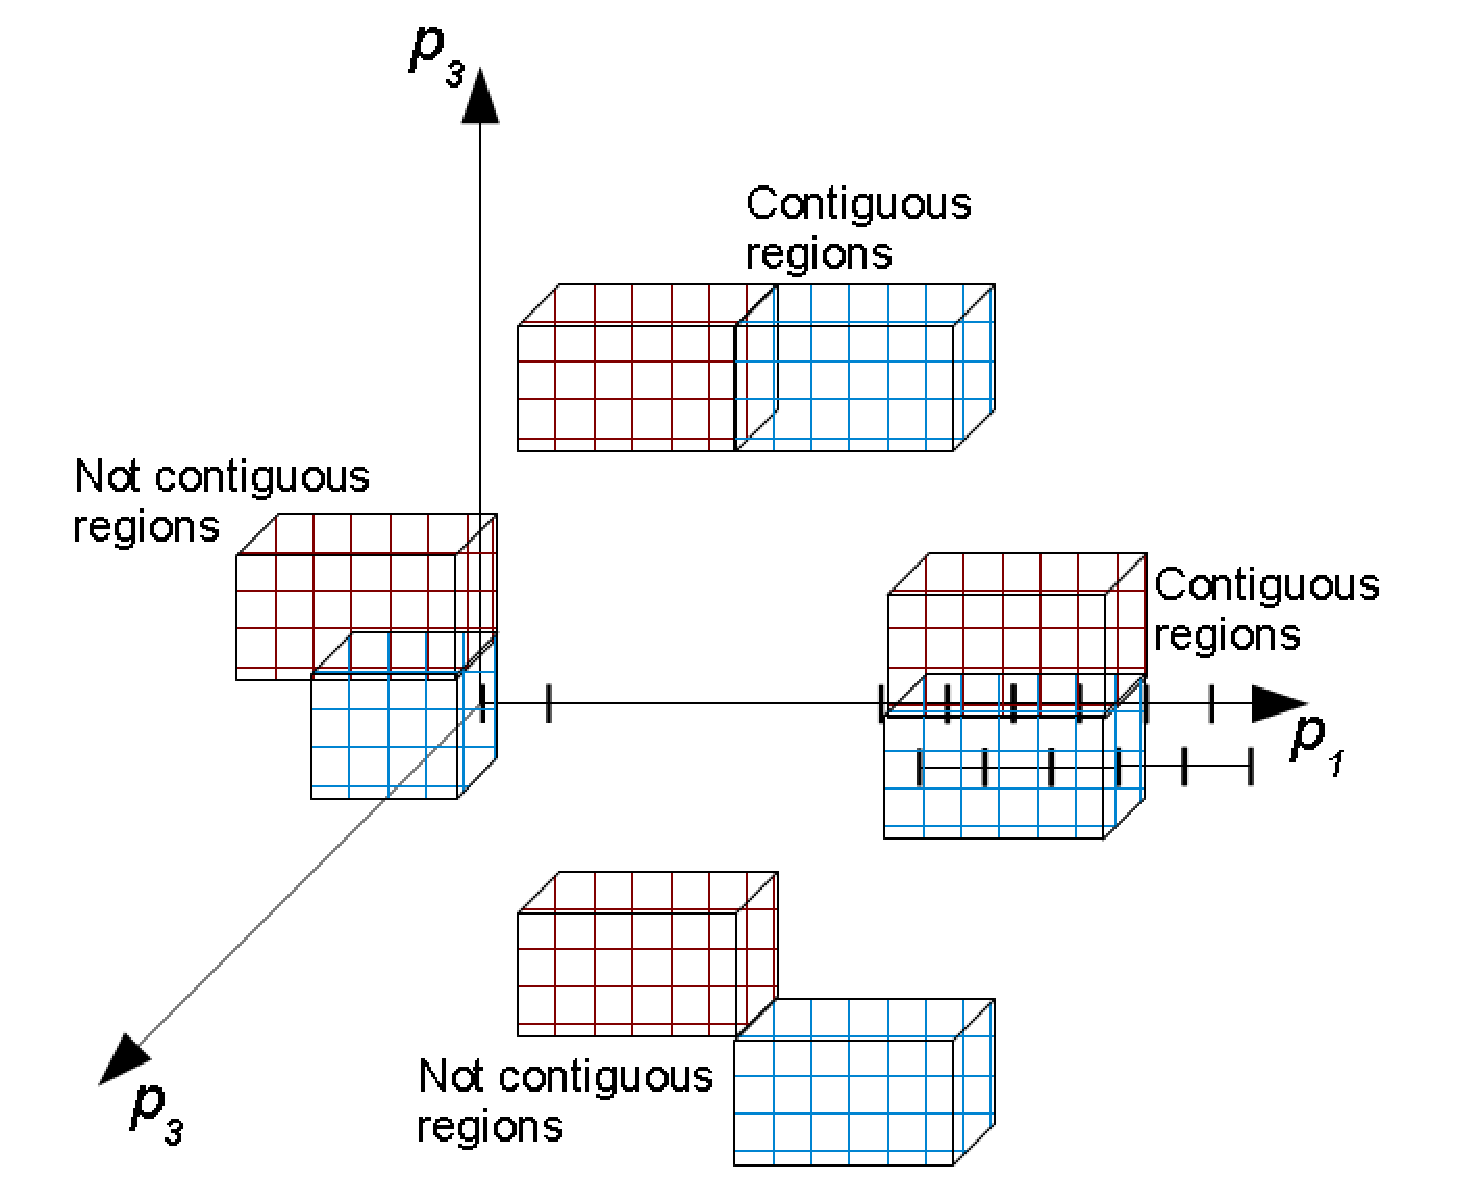
\includegraphics[width=0.9\columnwidth]{img/contiguous_regions}

\caption{\label{pers02.fig:Contiguous-regions}Contiguous and not contiguous
regions}
\end{figure}



\begin{defn}
\emph{\label{pers02.def:Merging-regions}Merging regions}

Let $R_{1}$ and $R_{2}$ be two contiguous regions as the previous
ones. Because of the definition of contiguous intervals, it is possible
that $b_{j}<x_{j}$ or $y_{j}<a_{j}$. We can merge the contiguous
intervals and obtain a new interval, as the following
\[
\left[t_{j},z_{j}\right]=\begin{cases}
\left[a_{j}..y_{j}\right] & \mbox{ if }b_{j}<x_{j}\\
\left[x_{j}..b_{j}\right] & \mbox{ if }y_{j}<a_{j}
\end{cases}
\]


The region ``$R_{1}$ merged with $R_{2}$'' is defined as
\[
R=\prod_{i<j}\left[a_{i}..b_{i}\right]\times\left[t_{j}..z_{j}\right]\times\prod_{i>j}\left[a_{i}..b_{i}\right]
\]


Such an $R$ will be indicated with the following notation:
\[
R=R_{1}+R_{2}
\]
\end{defn}
\begin{rem}
$R_{1}+R_{2}$ is mathematically equivalent to $R_{1}\cup R_{2}$.
However, using $R_{1}+R_{2}$ notation, we enforce the argument that
$R_{1}$ and $R_{2}$ must be to contiuguous regions.
\end{rem}

\begin{defn}
\emph{Separation}

Let $\mathbf{o}=\left(o_{1},\dots,o_{m}\right)$ and $\mathbf{q}=\left(q_{1},\dots,q_{m}\right)$
be two points of $O_{1}\times\dots\times O_{m}$. The separation between
$\mathbf{o}$ and $\mathbf{q}$ is 
\[
s\left(\mathbf{o}\rightarrow\mathbf{q}\right)=\sum_{i=1}^{m}\left|\frac{o_{i}-q_{i}}{o_{i}}\right|
\]


Notice that the separation is not a commutative operator.\end{defn}
\begin{rem}
The separation between $\mathbf{o}$ and $\mathbf{q}$ measures how
much we must vary $\mathbf{o}$ to transfrom it in $\mathbf{q}$.
The separation is a ``normalized'' measure that is independent of
the nature and the unit of measurement of the objectives
\end{rem}

\begin{defn}
\emph{Separation (alternative)}

Another definition of separation could be:
\[
s\left(\mathbf{o}\rightarrow\mathbf{q}\right)=\max_{i=1,\dots,m}\left|\frac{o_{i}-q_{i}}{o_{i}}\right|
\]

\end{defn}
